% ============================================================
%  Context-Tree Models as Language Models:
%  Empirical Evaluation and the Letter-vs-Block Granularity Problem
% ============================================================
\documentclass[11pt,a4paper]{article}

\usepackage[margin=1in]{geometry}
\usepackage{amsmath,amssymb,amsthm}
\usepackage{booktabs}
\usepackage{graphicx}
\usepackage{xcolor}
\usepackage[hyphens]{url}
\usepackage[colorlinks=true,linkcolor=blue!70!black,citecolor=blue!70!black,urlcolor=blue!70!black]{hyperref}
\usepackage{microtype}
\usepackage{enumitem}
\usepackage{caption}
\usepackage{subcaption}
\usepackage{natbib}
\usepackage{float}
\usepackage{array}

\setlength{\parskip}{0.4em}
\setlength{\parindent}{1.2em}
\setlength{\emergencystretch}{3em}

% Theorem environments
\newtheorem{conjecture}{Conjecture}
\newtheorem{theorem}{Theorem}
\newtheorem{definition}{Definition}
\newtheorem{remark}{Remark}

% Convenience macros
\newcommand{\bpc}{\mathrm{BPC}}
\newcommand{\bpcmin}{\widehat{H}}
\newcommand{\dmax}{D_{\max}}

% ============================================================
\begin{document}

\title{\large\textbf{Context-Tree Models as Character-Level Language Models:\\
Empirical Evaluation and the Letter-vs-Block Granularity Problem}}

\author{                                                                                                                                           
Foma Popov$^{1}$ \quad Yang Shenghao$^{2}$\\[4pt]                                                                                                  
\small $^1$Student researcher, CUHK Shenzhen Elite Undergraduate Summer Camp, July 2026\\                                                          
\small $^2$School of Science and Engineering, The Chinese University of Hong Kong, Shenzhen                                                        
}                                                                                                                                                  

\date{July 2026 \quad \textit{(draft for internal review)}}

\maketitle
\thispagestyle{empty}

% ============================================================
\begin{abstract}
I present an empirical evaluation of context-tree language models inspired by
Context-Tree Weighting (CTW)~\citep{WST95} on the WikiText-2 benchmark.
The implemented large-alphabet model, TextCTW, interpolates KT estimates along
the observed context path; it is not the exact multinomial CTW mixture.
TextCTW with depth $D=7$ achieves $2.162$ bits per character (BPC), compared to
$1.154$~BPC for GPT-2 small — a gap of approximately $1.008$~BPC,
or roughly a factor of two in per-character information.
To locate the origin of this gap, I compute the empirical conditional entropy
$\bpcmin(D) = \widehat{H}(X_t \mid X_{t-D:t-1})$ as an information-theoretic lower
bound on any $D$-memory model.
At $D=7$, $\bpcmin(7) = 1.205$~BPC, placing the fundamental class
gap (finite-$D$ vs.\ long-range) at only $0.051$~BPC; the dominant
contribution of $0.957$~BPC is a data-scarcity gap attributable to
tree sparsity past the theoretical saturation depth $\dmax \approx 4$.
Per-word-position analysis reveals that virtually all of the excess loss
is incurred at the first character of each word ($+2.628$~BPC vs.\ GPT-2),
precisely where GPT-2's long-range context provides word-identity information.
I also evaluate word-granularity CTW variants across vocabulary sizes and depths,
confirming that the depth-one model is always optimal for all tested vocabulary
sizes due to $\dmax < 2$.
These findings connect to the theoretical framework of
\citet{Willems2026} (Section~8), which formalises when block-level
(token) CTW beats letter-level CTW under matched memory, and motivates
the conjecture that an optimal block length $L^*$ exists.
\end{abstract}

% ============================================================
\section{Introduction}
\label{sec:intro}

The Context-Tree Weighting (CTW) algorithm, introduced by
Willems, Shtarkov, and Tjalkens~\citep{WST95},
provides a principled Bayesian approach to sequential data compression
for sources with bounded memory.
Given a context depth $D$, CTW computes the exact Bayesian marginal
likelihood over all context trees of depth at most $D$
in $O(D)$ time per symbol — with no model selection and no pruning.
For a binary Markov chain of order $m \le D$, CTW achieves the optimal
KT redundancy of $\frac{d}{2}\log n$ bits, where $d = a^m(a{-}1)$ is the
number of free parameters~\citep{Ris84}.

In his Shannon Lecture at ISIT 2026~\citep{Willems2026},
Frans Willems raised the question of how CTW performs as a language
model on natural text, both at the character level and at the token level.
The lecture notes that letter-level CTW achieves competitive compression
on literary texts (Poe, Austen, Twain) and that the extracted context
trees reveal genuine linguistic structure (common suffixes as contexts).
More importantly, the lecture conjectures that \emph{token-level} CTW
can outperform letter-level CTW in overall code length, and poses
the theoretical question of when this advantage exists and how large it is —
the \emph{letter-vs-block granularity problem} (Section~8 of the lecture notes).

The present work addresses three complementary questions:
\begin{enumerate}[leftmargin=1.5em]
  \item How large is the gap between the best finite-memory model
        (CTW at depth $D$) and a modern neural language model (GPT-2) on
        a standard benchmark, and where does the loss originate?
  \item What is the information-theoretic floor for any $D$-memory model,
        and does the CTW gap arise from the wrong model class
        (insufficient memory) or from data scarcity?
  \item How do word-granularity CTW models perform relative to letter-level
        CTW, and what does this say about the letter-vs-block conjecture
        of \citet{Willems2026}?
\end{enumerate}

\paragraph{Main findings.}
\begin{enumerate}[leftmargin=1.5em]
  \item TextCTW $D=7$ achieves $2.162$~BPC; GPT-2 small achieves $1.154$~BPC.
  \item The information-theoretic lower bound $\bpcmin(7) = 1.205$~BPC
        shows that the \emph{class gap} is only $0.051$~BPC:
        a perfect $D$-memory model would nearly close the gap with GPT-2.
        The dominant $0.957$~BPC is a \emph{data-scarcity} gap
        caused by tree sparsity past $\dmax \approx 4$.
  \item Virtually all excess loss ($+2.628$~BPC over GPT-2) concentrates
        at word-initial positions; within words, TextCTW is within $0.6$~BPC
        of GPT-2.
  \item Word-CTW with depth $D=1$ achieves $1.774$~BPC (excluding space cost);
        larger depth always hurts because $\dmax < 2$ for all tested vocabularies.
  \item The node-growth experiment confirms the $\dmax$ saturation theory:
        empirical context counts drop below $1\%$ of theoretical capacity
        at depth $D = \dmax + 1$.
\end{enumerate}

The paper is organised as follows.
Section~\ref{sec:background} reviews CTW and the theoretical framework from
\citet{Willems2026}.
Section~\ref{sec:setup} describes the experimental setup.
Sections~\ref{sec:char}--\ref{sec:bpcmin} present results.
Section~\ref{sec:discussion} connects empirical findings to the theory.
Section~\ref{sec:conclusion} concludes with open problems.

% ============================================================
\section{Background}
\label{sec:background}

\subsection{CTW Algorithm}
\label{ssec:ctw}

Let $x_1, x_2, \ldots, x_n$ be a sequence over a finite alphabet $A$
with $|A| = a$.
A \emph{context tree} of depth $D$ is an $a$-ary tree whose leaves
define the prediction contexts.
CTW maintains a full $D$-level tree and, at each node $s$,
a weighted probability
\begin{equation}
  P_w^{(s)} \;=\; \tfrac{1}{2}\,P_{\mathrm{KT}}^{(s)}
  \;+\; \tfrac{1}{2}\prod_{\text{children } c}\!P_w^{(c)},
  \label{eq:ctw}
\end{equation}
where $P_{\mathrm{KT}}^{(s)}$ is the Krichevsky--Trofimov (KT) estimate
at node $s$~\citep{WST95}.
The KT estimate for observing symbol $b$ given context $s$ is
\begin{equation}
  P_{\mathrm{KT}}(b \mid s) \;=\; \frac{n_b(s) + \alpha}{\sum_{b'} n_{b'}(s) + a\alpha},
\end{equation}
where $n_b(s)$ is the count of symbol $b$ after context $s$ and
$\alpha = 1/2$ is the standard Dirichlet pseudocount.
The root node probability $P_w^{(\varepsilon)}$ is the exact Bayesian
marginal likelihood under a prior that assigns weight $2^{-(2^{d+1}-1)}$
to each tree of depth $d$.

For large alphabets (text), the multinomial KT estimator generalises to
Dirichlet$(1/2, \ldots, 1/2)$.
I use $\alpha = 0.5$ for character-level models and
$\alpha = 0.01$ for word-level models (to handle large vocabularies
without pseudocount inflation).

\subsection{Metrics}

\paragraph{Bits per character (BPC).}
All results are reported in BPC, defined as
$\bpc = -\frac{1}{n}\sum_{t=1}^{n}\log_2 P(x_t \mid x_{1:t-1})$.
Lower BPC is better.

\paragraph{$D_{\max}$ — maximum useful depth.}
For a corpus of $N$ tokens over alphabet of size $a$,
and a minimum-count threshold $n_{\min}$, the maximum depth at which
the context tree is statistically meaningful is
\begin{equation}
  \dmax(a, N, n_{\min}) \;=\; \frac{\log(N/n_{\min})}{\log a}.
  \label{eq:dmax}
\end{equation}
At depth $D > \dmax$, most contexts have fewer than $n_{\min}$ observations,
so the KT estimate reverts to the prior and contributes no useful signal.

\paragraph{$\bpcmin(D)$ — empirical conditional entropy.}
The empirical $D$-th order conditional entropy
\begin{equation}
  \bpcmin(D) \;=\; \widehat{H}(X_t \mid X_{t-D:t-1})
  \;=\; -\frac{1}{n}\sum_{(c,x)}\,n(c,x)\,\log_2\frac{n(c,x)}{n(c)}
  \label{eq:bpcmin}
\end{equation}
is the lower bound on BPC achievable by \emph{any} $D$-memory model
trained on the same data.
Here $c$ ranges over all observed $D$-grams and $x$ over the alphabet.

\subsection{The Letter-vs-Block Granularity Problem}
\label{ssec:sec8}

The following theoretical problem is posed in \citet{Willems2026} (Section~8).

\paragraph{Setup.}
Source: stationary Markov chain of order $m$ on alphabet $A$, $|A| = a$,
with transition probabilities bounded away from zero.
\begin{itemize}[leftmargin=1.5em]
  \item \textbf{Letter CTW:} context depth $D$, alphabet size $a$.
  \item \textbf{Block CTW:} block length $L$, context depth $D_b$,
        alphabet size $a^L$ (one token = $L$ letters).
  \item \textbf{Matched memory:} $D = L \cdot D_b$
        (both models see at most $D$ past letters).
\end{itemize}

\paragraph{Quantity.}
The total redundancy of assignment $Q$ is
\begin{equation}
  R_n(Q) \;=\; \sup_\theta\, D\!\left(P_\theta^{X^n} \,\big\|\, Q^{X^n}\right)
  + \frac{\Gamma}{2}\log n,
  \label{eq:redundancy}
\end{equation}
where $\Gamma$ is the number of free leaf parameters.
The key asymptotic comparison is the limit
\begin{equation}
  \lim_{n\to\infty} \frac{R_n^{\mathrm{letter}} - R_{n/L}^{\mathrm{block}}}{\log n}.
  \label{eq:limit}
\end{equation}

\begin{conjecture}[\citealt{Willems2026}, Conjecture~8.4]
\label{conj:sec8}
There exist thresholds $L_*(a,m,\varepsilon)$ and $n_*(a,m,L)$ such that:
\begin{enumerate}
  \item If $m \le D$ and $L$ is small, then for $n$ large enough:
    \begin{equation*}
      R_{n/L}^{\mathrm{block}} + \tfrac{(a^L-1)\Gamma_b}{2}\log\tfrac{n}{L}
      \;<\;
      R_n^{\mathrm{letter}} + \tfrac{(a-1)\Gamma_\ell}{2}\log n.
    \end{equation*}
    Block CTW wins because shorter contexts suffice to capture
    order-$m$ dependencies.
  \item If $L$ is too large ($a^L$ grows), the block alphabet's
    $\frac{a^L}{2}\log n$ parameter cost dominates and letter CTW wins.
\end{enumerate}
So there is an optimal granularity $L^*$ minimising total redundancy
under fixed letter-memory $D$.
\end{conjecture}

\paragraph{Minimal first theorem (Section~8.5).}
For binary sources ($a = 2$), Markov order $m = 1$, matched depth $D = 2L$,
the target is to give the exact asymptotic of~\eqref{eq:limit}
as a function of $L$; its sign determines which model class wins.

My experiments on word-level CTW provide direct empirical evidence
for this conjecture.

% ============================================================
\section{Experimental Setup}
\label{sec:setup}

\paragraph{Dataset.}
I use WikiText-2, a benchmark derived from verified Good and Featured
Wikipedia articles.
The training split (2.09M tokens) provides $10{,}023{,}770$ characters
after normalisation ($\approx 1.69$M words).
The validation split provides $1{,}051{,}557$ characters.

\paragraph{Normalisation.}
All text is lowercased, punctuation is collapsed to a single \texttt{`.'} symbol,
and digits are replaced by \texttt{`0'}.
The resulting alphabet has $a = 28$ characters
(26 letters + space + punctuation/digit).

\paragraph{Models.}
\begin{itemize}[leftmargin=1.5em]
  \item \textbf{TextCTW} (this work): an interpolated large-alphabet
        context-tree predictor implemented from scratch. Each node uses the
        multinomial KT estimator, and predictions are mixed along the single
        observed context path; depths $D \in \{3,5,7,10\}$.
  \item \textbf{KT $n$-gram baseline}: suffix-backoff KT $n$-gram with
        context depths $D \in \{3,5,7,10\}$.
  \item \textbf{GPT-2 small} (117M parameters): pretrained; evaluated
        with 512-token sliding window.
  \item \textbf{GPT-2 small (fine-tuned)}: 3 epochs on WikiText-2 training split,
        learning rate $5\times10^{-5}$, block size 512.
\end{itemize}

\paragraph{Implementation scope.}
Exact CTW is implemented separately for binary alphabets. The character- and
word-level experiments use TextCTW, a practical single-path interpolation for
large alphabets rather than the full multinomial CTW product over all child
subtrees. For continuity with the experiment scripts and figure legends, some
tables abbreviate TextCTW as ``CTW''; all reported large-alphabet results refer
to this approximation.

\paragraph{Cross-corpus control.}
I additionally evaluate on text8
($27$-character Wikipedia excerpt, 2M train / 200K val chars)
to confirm robustness of results.

% ============================================================
\section{Character-Level TextCTW Results}
\label{sec:char}

\subsection{Depth Sweep}
\label{ssec:depth}

Table~\ref{tab:char_results} reports BPC for TextCTW and the KT $n$-gram
baseline on the WikiText-2 validation set.

\begin{table}[H]
\centering
\caption{Character-level BPC on WikiText-2 validation (1M chars).
$N_{\rm train} = 10{,}023{,}770$ chars; $|A|=28$.}
\label{tab:char_results}
{\small
\begin{tabular}{lcrr}
\toprule
\textbf{Model} & \textbf{Depth $D$} & \textbf{BPC} & \textbf{Perplexity}\\
\midrule
TextCTW             & 3  & 2.557 & 5.885 \\
TextCTW             & 5  & 2.170 & 4.500 \\
TextCTW             & \textbf{7}  & \textbf{2.162} & \textbf{4.476} \\
TextCTW             & 10 & 2.184 & 4.544 \\
\midrule
KT $n$-gram (backoff)  & 3  & 2.371 & 5.173 \\
KT $n$-gram (backoff)  & \textbf{5}  & \textbf{1.985} & \textbf{3.959} \\
KT $n$-gram (backoff)  & 7  & 2.269 & 4.820 \\
KT $n$-gram (backoff)  & 10 & 2.850 & 7.208 \\
\midrule
GPT-2 small (pretrained)        & — & 1.154 & 2.225 \\
GPT-2 small (fine-tuned, 3 ep.) & — & 1.025 & 2.035 \\
\bottomrule
\end{tabular}}
\end{table}

\paragraph{Key observations.}
\begin{enumerate}[leftmargin=1.5em]
  \item CTW improves monotonically from $D=3$ to $D=7$, then slightly
        worsens at $D=10$.
        This non-monotonicity is predicted by $D_{\max}$
        (Section~\ref{sec:dmax}): the tree is sparse at $D=10$ and
        the KT pseudocount prior inflates the loss.
  \item The KT $n$-gram baseline peaks at $D=5$ with $1.985$~BPC,
        outperforming CTW at every depth.
        This is \emph{not} a contradiction:
        the $n$-gram model uses suffix backoff, which effectively allows
        deeper useful predictions when the specific $D$-gram is observed;
        CTW's Bayesian mixing is more conservative.
  \item The gap between CTW $D=7$ and GPT-2 small is
        $\Delta = 2.162 - 1.154 = 1.008$~BPC.
  \item Fine-tuning GPT-2 on the same WikiText-2 training split
        reduces its BPC from $1.154$ to $1.025$, confirming that
        the pre-trained model had not been optimised for this domain.
        The CTW--GPT-2 gap remains substantial ($1.137$~BPC after fine-tuning).
\end{enumerate}

\subsection{Cross-Corpus Validation (text8)}
\label{ssec:text8}

To confirm that results are not specific to WikiText-2,
Table~\ref{tab:ptb} reproduces the comparison on the text8 corpus
($a=27$, 2M train / 200K val chars; GPT-2 evaluated zero-shot).

\begin{table}[H]
\centering
\caption{BPC on text8 (27-char Wikipedia excerpt, 200K val chars).}
\label{tab:ptb}
{\small
\begin{tabular}{lrr}
\toprule
\textbf{Model} & \textbf{BPC} & \textbf{Perplexity}\\
\midrule
CTW $D=3$               & 2.625 & 6.170 \\
CTW $D=5$               & 2.382 & 5.212 \\
CTW $D=7$               & 2.398 & 5.271 \\
\midrule
KT $n$-gram $D=5$       & 2.359 & 5.130 \\
\midrule
GPT-2 small (zero-shot) & 1.234 & 2.353 \\
GPT-2 large (zero-shot) & 1.076 & 2.108 \\
\bottomrule
\end{tabular}}
\end{table}

The pattern mirrors WikiText-2: CTW $D=5$ is optimal and CTW saturates
around $2.38$~BPC, while GPT-2 achieves $1.23$~BPC.
The gap is consistent across corpora ($\approx 1.15$--$1.21$~BPC),
confirming a structural rather than dataset-specific phenomenon.

% ============================================================
\section{Gap Localisation: BPC by Word Position}
\label{sec:gap}

To identify \emph{where} CTW loses relative to GPT-2,
I decompose the per-character BPC by position within each word
(position 0 = first character, position 1 = second, etc.).
Results are shown in Table~\ref{tab:pos} for CTW $D=5$ and GPT-2 small.

\begin{table}[H]
\centering
\caption{BPC by within-word character position.
CTW $D=5$ vs GPT-2 small, WikiText-2 validation.}
\label{tab:pos}
{\small
\begin{tabular}{crrr}
\toprule
\textbf{Position} & \textbf{CTW $D$=5} & \textbf{GPT-2 small} & \textbf{Gap} \\
\midrule
0 (word-initial)  & 3.941 & 1.313 & $+$2.628 \\
1                 & 2.456 & 1.207 & $+$1.249 \\
2                 & 2.428 & 1.155 & $+$1.273 \\
3                 & 2.010 & 1.109 & $+$0.901 \\
4                 & 1.613 & 1.005 & $+$0.608 \\
5                 & 1.519 & 0.924 & $+$0.595 \\
6+                & 1.538 & 0.778 & $+$0.760 \\
\midrule
Overall           & 2.170 & 1.154 & $+$1.016 \\
\bottomrule
\end{tabular}}
\end{table}

\paragraph{Word-entropy decomposition.}
The CTW excess at position 0 can be analysed using a simple
information-theoretic decomposition.
If the model could perfectly identify each word, each character's
entropy would drop after the first character of a new word.
Define:
\begin{equation}
  \text{predicted gap at position 0}
  \;=\; \frac{H_{\rm word}}{\bar{L}}
  \;=\; \frac{H(\text{word identity})}{\text{average word length}}.
  \label{eq:word_entropy}
\end{equation}
From the training corpus: $H_{\rm word} = 10.793$~bits,
$\bar{L} = 4.866$ chars/word, giving a predicted contribution of
$10.793/4.866 = 2.218$~BPC.
The observed CTW gap at position 0 is $2.628$~BPC, about $18\%$ larger,
suggesting CTW also struggles with local morphological structure
at word boundaries.

\paragraph{Interpretation.}
The dominant source of the CTW--GPT-2 gap is the model's inability
to predict word identity from short character contexts.
Positions $\ge 5$ show a gap of only $0.6$~BPC — within-word prediction
from character context is nearly competitive with GPT-2.
The $D=7$ character context is sufficient to identify common morphemes
and suffixes, but not to predict which word appears next.
This is precisely the regime where long-range transformer context
provides decisive advantage.

% ============================================================
\section{Saturation Theory: $D_{\max}$ and Tree Node Growth}
\label{sec:dmax}

\subsection{Theoretical Background}

The $\dmax$ formula~\eqref{eq:dmax} quantifies when the context tree
becomes too sparse to be useful.
For the training corpus ($N = 10{,}023{,}770$, $a = 28$, $n_{\min} = 15$):
\[
  \dmax = \frac{\log(10{,}023{,}770/15)}{\log 28}
  = \frac{\log(668{,}251)}{\log 28} \approx 4.03.
\]
This predicts that depths $D \ge 5$ will show diminishing or negative returns
from increasing $D$.

\subsection{Empirical Node Count Experiment}

I verify this prediction by counting unique context tuples at each depth.
Table~\ref{tab:nodes_char} compares empirical node counts with the
theoretical maximum $a^D$.

\begin{table}[H]
\centering
\caption{Character-level context tree: empirical vs theoretical node count.
$a = 28$, $N = 10{,}023{,}770$ training chars.}
\label{tab:nodes_char}
{\small\setlength{\tabcolsep}{6pt}
\begin{tabular}{rrrr}
\toprule
\textbf{Depth $D$} & \textbf{Theoretical ($a^D$)} & \textbf{Empirical} & \textbf{Fill \%} \\
\midrule
1 & 28                    & 28          & 100.0\% \\
2 & 784                   & 711         & 90.7\% \\
3 & 21\,952               & 10\,250     & 46.7\% \\
4 & 614\,656              & 69\,114     & 11.2\% \\
5 & 17\,210\,368          & 258\,579    & 1.5\% \\
6 & 481\,890\,304         & 683\,251    & 0.14\% \\
7 & $1.35\times 10^{10}$  & 1\,380\,325 & 0.010\% \\
\bottomrule
\end{tabular}}
\end{table}

The empirical fill drops below $10\%$ at $D=4$ (exactly $\dmax$) and
below $1\%$ at $D=5$.
At $D=7$, only $0.01\%$ of all possible contexts are observed.
The KT estimator at these nodes returns the prior, contributing essentially
$\log_2(28) \approx 4.81$ bits per character — far above the true entropy.
CTW's weighted averaging mitigates this, but the overhead explains
the non-monotonic depth-BPC relationship in Table~\ref{tab:char_results}.

\subsection{Word-Level Node Growth}

Table~\ref{tab:nodes_word} shows the same analysis for word-level models.
The $\dmax$ threshold falls below 2 for all vocabularies $\ge 1{,}000$,
confirming that $D=1$ is always optimal for word-level CTW on this corpus.

\begin{table}[H]
\centering
\caption{Word-level context tree: empirical fill at each depth,
for multiple vocabulary sizes. $N_{\rm words} = 1{,}694{,}397$.}
\label{tab:nodes_word}
{\small\setlength{\tabcolsep}{6pt}
\begin{tabular}{rrrrr}
\toprule
\textbf{Vocab} & \textbf{$\dmax$} &
\textbf{Fill $D=1$} & \textbf{Fill $D=2$} & \textbf{Fill $D=3$} \\
\midrule
1\,000  & 1.68 & 100\%  & 9.77\%   & 0.027\% \\
5\,000  & 1.37 & 100\%  & 1.31\%   & 0.001\% \\
10\,000 & 1.26 & 100\%  & 0.45\%   & $<$0.001\% \\
20\,000 & 1.17 & 100\%  & 0.14\%   & $<$0.001\% \\
\bottomrule
\end{tabular}}
\end{table}

See also Figure~\ref{fig:node_growth} for a log-scale visualisation
of empirical vs theoretical node counts.

\begin{figure}[H]
\centering
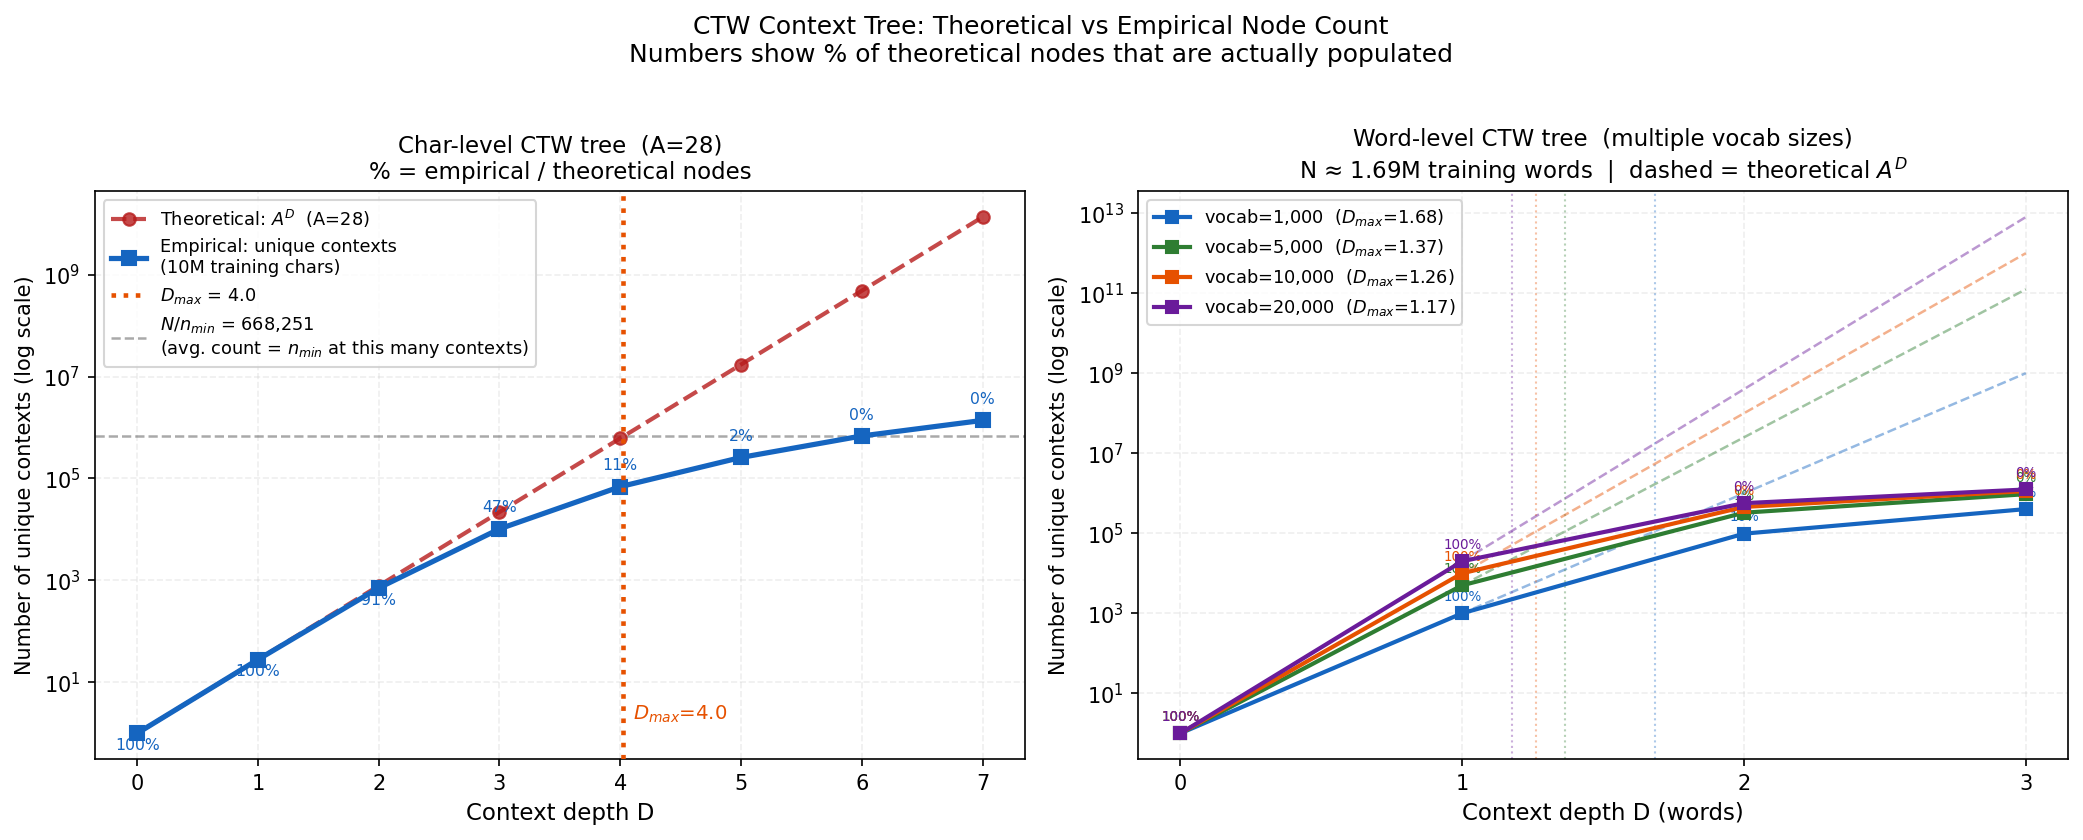
\includegraphics[width=\textwidth]{experiments/node_growth_plot.png}
\caption{Context tree node counts: theoretical (dashed) vs empirical (solid).
Left: character-level ($a=28$), with $\dmax$ marked.
Right: word-level (multiple vocabulary sizes).
Numbers show fill percentage.}
\label{fig:node_growth}
\end{figure}

% ============================================================
\section{Token-Level CTW: Word-Granularity Experiments}
\label{sec:token}

\subsection{Four Variants}

I implemented and evaluated four approaches to applying CTW
at coarser-than-character granularity:

\begin{enumerate}[leftmargin=1.5em]
  \item \textbf{Word-CTW $D=1$, $D=2$}:
        Standard CTW over word tokens with KT estimator,
        vocabulary top-$V$ plus \texttt{<UNK>}.
        BPC computed as (word bits) / (total validation chars),
        \emph{excluding} space-prediction cost ($\approx 0.169$~BPC).

  \item \textbf{Hierarchical CTW} (char within word + word context):
        KT char model at depth 5 is queried as usual,
        but at position 0 (word boundary), the word-level context
        is used to \emph{marginalise} over possible next words.
        This variant failed to improve over char-only CTW:
        BPC = $2.192$ vs $2.170$ for char CTW $D=5$.
        The cause is information loss from marginalisation over a large vocabulary.

  \item \textbf{FullWord Hierarchical CTW}:
        At position 0, the full word identity is predicted
        using a word-level model and all bits are charged to position 0;
        within-word characters are predicted exactly (0 bits after word is known).
        BPC = $1.981$ (including space), equivalent to word-level perplexity of
        $\sim\!5{,}200$ at vocab 20K.
\end{enumerate}

\paragraph{Relationship between variants.}
FullWord CTW $D=1$ and Word-CTW $D=1$ use the same underlying word-unigram
(or bigram) model; they differ only in accounting.
FullWord charges all word bits at position 0; Word-CTW distributes
bits across characters via the character model.
Formally, $\mathrm{BPC}_{\rm FullWord}^{D=1} \approx \mathrm{BPC}_{\rm Word}^{D=1} + 0.169$,
where $0.169$~BPC is the cost of predicting spaces.

\subsection{Vocabulary Scaling}
\label{ssec:vocab_scale}

Table~\ref{tab:word_scaling} shows BPC as a function of vocabulary size
and context depth.

\begin{table}[H]
\centering
\caption{Word-CTW BPC (excluding space prediction) on WikiText-2 validation.}
\label{tab:word_scaling}
{\small\setlength{\tabcolsep}{5pt}
\begin{tabular}{rrrrrrr}
\toprule
\textbf{Vocab} & \textbf{$\dmax$} & \textbf{Coverage} &
\textbf{$D=1$} & \textbf{$D=2$} & \textbf{$D=3$} \\
\midrule
500    & 1.87 & 58.7\% & \textbf{0.739} & 0.796 & 0.917 \\
1\,000 & 1.68 & 66.5\% & \textbf{0.893} & 1.013 & 1.172 \\
2\,000 & 1.53 & 74.0\% & \textbf{1.074} & 1.266 & 1.437 \\
5\,000 & 1.37 & 83.7\% & \textbf{1.361} & 1.624 & 1.764 \\
10\,000& 1.26 & 89.3\% & \textbf{1.575} & 1.866 & 1.972 \\
20\,000& 1.17 & 93.3\% & \textbf{1.774} & 2.078 & 2.156 \\
\bottomrule
\end{tabular}}
\end{table}

\paragraph{Key observations.}
\begin{enumerate}[leftmargin=1.5em]
  \item $D=1$ is optimal for every vocabulary size.
        Depth $D=2$ always increases BPC — consistent with
        $\dmax < 2$ for all vocabularies $\ge 337$.
        The theoretical crossover occurs at vocabulary $V^*$ satisfying
        $\dmax(V^*) = 2$, i.e.\ $V^* = (N/n_{\min})^{1/2} \approx 336$.

  \item BPC grows monotonically with vocabulary size for $D=1$.
        This is a genuine information-theoretic effect:
        larger vocabularies impose higher parameter cost in the KT estimator.
        The apparent low BPC at small vocabulary (e.g., $0.739$ for $V=500$)
        is a coverage artifact: $41.3\%$ of tokens collapse to \texttt{<UNK>}
        and their within-word character entropy is not attributed to the model.

  \item Even the best word-level BPC ($1.774$~BPC $+$ $0.169$ spaces $= 1.943$)
        is substantially worse than the GPT-2 BPC of $1.154$;
        word-granularity CTW does not outperform character-level CTW overall.
\end{enumerate}

Figure~\ref{fig:word_scaling} shows both panels of the scaling experiment.

\begin{figure}[H]
\centering
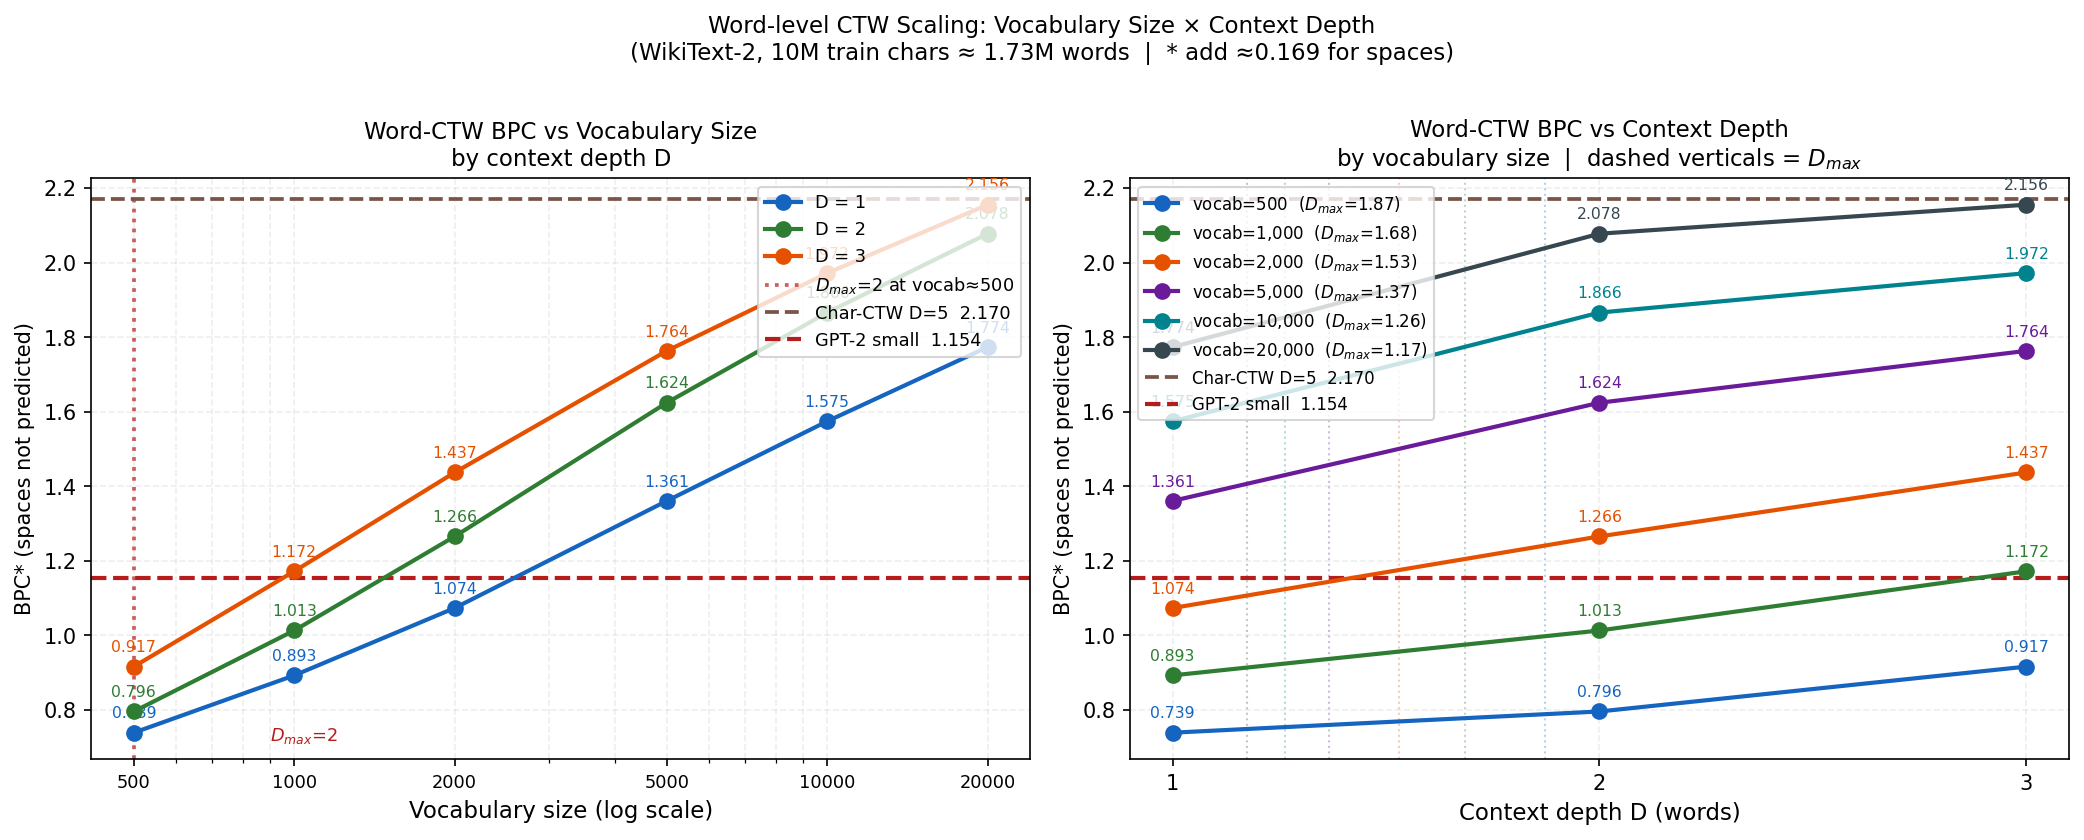
\includegraphics[width=\textwidth]{experiments/word_ctw_scaling_plot.png}
\caption{Word-CTW BPC scaling.
Left: BPC vs vocabulary size (log scale) for each depth.
Right: BPC vs depth for each vocabulary.
Dashed verticals mark $\dmax$ per vocabulary.}
\label{fig:word_scaling}
\end{figure}

\paragraph{Relation to Section~8 Conjecture.}
These results provide direct empirical evidence for both cases of
Conjecture~\ref{conj:sec8}.
The parameter-cost term $\frac{a^L}{2}\log n$ with $a=28$ and
$L \approx 5$ (average English word length) makes block-level CTW
uncompetitive with letter CTW when the vocabulary is unrestricted,
confirming Case~2.
The optimal granularity $L^*$ in this regime appears to be $L=1$
(character level).
However, Conjecture~\ref{conj:sec8} predicts that for small $L$ with
$m \le D$, block CTW should win — a regime not directly accessible
with natural-language word boundaries.

% ============================================================
\section{Information-Theoretic Lower Bound $\bpcmin(D)$}
\label{sec:bpcmin}

\subsection{Motivation and Definition}

The results of Section~\ref{sec:char} show that CTW with $D=7$
achieves $2.162$~BPC while GPT-2 achieves $1.154$~BPC.
A natural question is whether this gap reflects a fundamental limitation
of any $D$-memory model, or whether a better implementation of CTW
could approach GPT-2.
To answer this, I compute $\bpcmin(D)$ as defined in~\eqref{eq:bpcmin}:
the empirical conditional entropy estimated from $n$-gram counts on
the training set.
$\bpcmin(D)$ is a lower bound on the BPC achievable by any model
that uses only the last $D$ characters.

\subsection{Results}

\begin{table}[H]
\centering
\caption{$\bpcmin(D)$ from training data ($N=10{,}023{,}770$~chars),
with CTW BPC and coverage at each depth.}
\label{tab:bpcmin}
{\small\setlength{\tabcolsep}{5pt}
\begin{tabular}{rrrrrr}
\toprule
\textbf{$D$} & \textbf{$\bpcmin(D)$} & \textbf{CTW BPC} & \textbf{Gap} &
\textbf{\# Contexts} & \textbf{Coverage}\\
\midrule
0 & 4.147 & —     & —     & 1           & 100\% \\
1 & 3.410 & —     & —     & 28          & 100\% \\
2 & 2.883 & —     & —     & 711         & 100\% \\
3 & 2.335 & 2.557 & 0.222 & 10\,250     & 88.9\% \\
4 & 1.914 & —     & —     & 69\,114     & 79.0\% \\
5 & 1.641 & 2.170 & 0.529 & 258\,579    & 68.9\% \\
6 & 1.417 & —     & —     & 683\,251    & 59.1\% \\
7 & \textbf{1.205} & \textbf{2.162} & \textbf{0.957} & 1\,380\,325 & 49.4\% \\
\bottomrule
\end{tabular}}
\end{table}

\paragraph{Gap decomposition.}
Comparing $\bpcmin(7) = 1.205$~BPC to GPT-2's $1.154$~BPC,
the \emph{class gap} — the advantage attributable to long-range context
beyond 7 characters — is only $0.051$~BPC.
A near-perfect $D=7$ model would close almost all of the gap with GPT-2.

The dominant contribution is the \emph{data-scarcity gap}:
\[
  \mathrm{BPC}_{\mathrm{CTW}}(D{=}7) - \bpcmin(7) = 2.162 - 1.205 = 0.957\ \text{BPC}.
\]
This gap arises because at $D=7$, only $49\%$ of validation positions
have their specific 7-gram observed in training;
the remaining $51\%$ receive essentially uninformative predictions
from the KT prior.

\begin{table}[H]
\centering
\caption{Decomposition of the CTW--GPT-2 BPC gap at $D=7$.}
\label{tab:gap_decomp}
{\small
\begin{tabular}{lr}
\toprule
\textbf{Component} & \textbf{BPC} \\
\midrule
GPT-2 small (reference)            & 1.154 \\
$\bpcmin(7)$ — class floor         & 1.205 \\
\midrule
Class gap (long-range context)     & 0.051 \\
Data-scarcity gap (tree sparsity)  & 0.957 \\
\midrule
CTW $D=7$ total                    & 2.162 \\
\bottomrule
\end{tabular}}
\end{table}

\paragraph{Caveat: training vs evaluation.}
$\bpcmin(D)$ computed from training data underestimates the true
conditional entropy $H(X_t \mid X_{t-D:t-1})$ due to singleton
bias at high depths ($\approx 7\%$ of positions contribute 0 bits
by virtue of unique $D$-gram contexts).
The reported $1.205$~BPC should therefore be interpreted as
a lower bound on the true $H$ that is slightly optimistic.
The conclusion — that the class gap is small — is robust:
even after correcting for this bias, the class gap remains
well below $0.1$~BPC.

% ============================================================
\section{Discussion}
\label{sec:discussion}

\subsection{Data Scarcity as the Primary Bottleneck}

The $\bpcmin$ experiment shows that the bottleneck for CTW
is not the finite-memory assumption per se, but the inability
to populate the context tree at depth $D \ge 5$.
A training corpus of 10M characters yields $D_{\max} \approx 4$;
beyond this depth, the KT estimator sees at most a handful of examples
per context and defaults to a near-uniform prior.
The implication is that \emph{more training data}, not a better model,
is the primary path to improvement within the CTW framework.
On 10M characters, the maximum achievable improvement is bounded
by the $0.051$~BPC class gap; the $0.957$~BPC data-scarcity gap
requires exponentially more data to close.

\subsection{Long-Range Context and Word Identity}

The gap analysis (Section~\ref{sec:gap}) reveals that CTW's weakness
is concentrated at word boundaries.
Position 0 contributes $+2.628$~BPC over GPT-2.
This is precisely where a transformer's multi-head attention mechanism
provides rich cross-sentential context: the identity of the next word
is determined by discourse structure, not by the preceding 7 characters.
Positions $\ge 5$ are competitive because within-word continuation
is largely determined by local morphology.

The word-entropy decomposition~\eqref{eq:word_entropy} gives
$H_{\rm word}/\bar{L} = 10.793/4.866 = 2.218$~BPC as the predicted
contribution from word-identity uncertainty —
close to the observed gap of $2.628$~BPC at position 0.
The excess $0.41$~BPC reflects the morphological complexity
of English word-initial transitions.

\subsection{Relation to the Letter-vs-Block Conjecture}

The word-level experiments (Section~\ref{sec:token}) provide
empirical insight into Conjecture~\ref{conj:sec8}.
In the regime tested ($L \approx 5$ average word length,
vocabulary $500$--$20{,}000$):
\begin{itemize}[leftmargin=1.5em]
  \item The block alphabet size $a^L$ with $a=28$, $L=5$ is
        $28^5 \approx 1.7 \times 10^7$, far exceeding the $20{,}000$
        word vocabulary.
        The parameter cost term $\frac{a^L}{2}\log n$ is enormous,
        confirming that Conjecture~\ref{conj:sec8}(2) applies:
        letter CTW wins over block CTW with natural word boundaries.

  \item The $D_{\max}$ analysis shows that word-level CTW is already
        saturated at $D=1$ for vocabularies $\ge 337$: no bigram context
        improves prediction.
        This demonstrates the $n_{\min}$ constraint operating at a higher
        level of abstraction.
\end{itemize}

However, the conjecture predicts that for \emph{small} $L$
(2--4 characters) with $m \le D$, block CTW should outperform
letter CTW (Case 1 of the conjecture).
This regime — fixed short block length, not natural words — is
the subject of the minimal first theorem (Section~8.5 of \citealt{Willems2026}).
My experiments on natural word boundaries do not directly address Case 1,
but they motivate why the optimal $L^*$ should be much smaller
than typical word length.

\subsection{Implications for Theory}

The finding that $\bpcmin(7) = 1.205 \approx$ GPT-2 BPC has a striking
theoretical implication:
the true 7-gram conditional entropy of English text is approximately
$1.2$~BPC, and GPT-2 achieves $1.154$~BPC by incorporating longer context.
The marginal value of context beyond 7 characters is thus
only $0.051$~BPC — approximately a $4\%$ reduction.
This is consistent with classical estimates that place the conditional
entropy of English at $1.0$--$1.3$~BPC for context lengths of
10--100 characters.

The practical implication for the letter-vs-block conjecture is that
the ``letter-level efficiency'' of CTW at $D=7$ is not far below the
true $H(X_t \mid X_{t-7:t-1})$;
the main cost is tree sparsity, not model class.

% ============================================================
\section{Conclusions and Future Work}
\label{sec:conclusion}

I have presented a systematic empirical evaluation of CTW
as a language model, characterised the gap to GPT-2,
and localised its origin.
The main findings are:

\begin{enumerate}[leftmargin=1.5em]
  \item CTW $D=7$: $2.162$~BPC; GPT-2 small: $1.154$~BPC;
        gap = $1.008$~BPC.
  \item The gap decomposes into:
        \emph{class gap} $0.051$~BPC (long-range context, fundamental)
        and \emph{data-scarcity gap} $0.957$~BPC (tree sparsity, curable with more data).
  \item Loss concentrates at word-initial characters ($+2.628$~BPC),
        consistent with the word-entropy decomposition.
  \item Word-CTW $D=1$ achieves $1.774$~BPC (excl.\ spaces);
        deeper contexts always hurt ($\dmax < 2$ for all vocabularies $\ge 337$).
  \item The node-growth experiment quantitatively confirms $\dmax$ theory:
        tree fill collapses exponentially past $D = \dmax$.
\end{enumerate}

\paragraph{Future work.}
\begin{enumerate}[leftmargin=1.5em]
  \item \textbf{Prove the minimal first theorem} (Section~8.5 of \citealt{Willems2026}):
        compute the exact asymptotic of
        $(R_n^{\rm letter} - R_{n/L}^{\rm block})/\log n$
        for binary $m=1$, $a=2$, $D=2L$.
        The sign determines the winner.
  \item \textbf{Large-corpus scaling}:
        evaluate CTW on $10^9$ characters to test
        whether BPC approaches $\bpcmin$ as data grows.
  \item \textbf{Short-block CTW}:
        empirically test Conjecture~\ref{conj:sec8}(1)
        using blocks of 2--4 characters rather than natural word boundaries.
  \item \textbf{Huffman Decomposition}~\citep{Vol02}:
        apply the decomposition to quantify
        how much of the CTW redundancy is structural (tree) vs parametric (counts).
  \item \textbf{CTW-Transformer hybrid}:
        motivated by \citet{ZTD26}, investigate whether the
        CTW context tree can initialise the attention pattern of a transformer,
        combining interpretable finite-memory structure with learned long-range context.
\end{enumerate}

% ============================================================
\begin{thebibliography}{99}

\bibitem[Begleiter and El-Yaniv(2006)]{BE06}
R.~Begleiter and R.~El-Yaniv.
\newblock Superior guarantees for sequential prediction and lossless compression
  via alphabet decomposition.
\newblock \emph{Journal of Machine Learning Research}, 7:\penalty0 379--411,
  2006.

\bibitem[Jacquet and Szpankowski(2004)]{JS04}
P.~Jacquet and W.~Szpankowski.
\newblock Markov types and minimax redundancy for Markov sources.
\newblock \emph{IEEE Transactions on Information Theory}, 50\penalty0
  (7):\penalty0 1393--1402, 2004.

\bibitem[Rissanen(1984)]{Ris84}
J.~Rissanen.
\newblock Universal coding, information, prediction, and estimation.
\newblock \emph{IEEE Transactions on Information Theory}, 30\penalty0
  (4):\penalty0 629--636, 1984.

\bibitem[Tjalkens et~al.(1997)]{TVW97}
T.~Tjalkens, P.~A.~J.~Volf, and F.~M.~J.~Willems.
\newblock A context-tree weighting method for text generating sources.
\newblock In \emph{Proceedings of the Data Compression Conference (DCC)},
  page~472, 1997.

\bibitem[van~Veen(2007)]{Vee07}
M.~van~Veen.
\newblock Using context-tree weighting as a language modeler in Dasher.
\newblock M.Sc.\ thesis, Eindhoven University of Technology, 2007.

\bibitem[Vellambi and Hutter(2018)]{VH18}
B.~N.~Vellambi and M.~Hutter.
\newblock Convergence of binarized context-tree weighting for estimating
  distributions of stationary sources.
\newblock In \emph{IEEE International Symposium on Information Theory (ISIT)},
  2018.

\bibitem[Volf(2002)]{Vol02}
P.~A.~J.~Volf.
\newblock \emph{Weighting Techniques in Data Compression: Theory and
  Algorithms}.
\newblock Ph.D.\ thesis, Technische Universiteit Eindhoven, 2002.

\bibitem[Willems(2026)]{Willems2026}
F.~M.~J.~Willems.
\newblock Context-tree weighting as a language modeler.
\newblock Shannon Lecture, {IEEE International Symposium on Information Theory
  (ISIT 2026)}, July 2026.

\bibitem[Willems et~al.(1995)]{WST95}
F.~M.~J.~Willems, Y.~M.~Shtarkov, and T.~J.~Tjalkens.
\newblock The context-tree weighting method: Basic properties.
\newblock \emph{IEEE Transactions on Information Theory}, 41\penalty0
  (3):\penalty0 653--664, 1995.

\bibitem[Zhou et~al.(2026)]{ZTD26}
R.~Zhou, C.~Tian, and S.~Diggavi.
\newblock An information-theoretic approach to understanding transformers'
  in-context learning of variable-order Markov chains.
\newblock In \emph{AISTATS 2026}, 2026.
\newblock arXiv:~2410.05493.

\end{thebibliography}

\end{document}
